\chapter{Design and Implementation}
\label{chap:implementation}
Talk about design choices such as only multiple choices, no exercises asking to write code, writing custom server, etc...

Mention three tier architecture

implemented as a JavaFx applet
javafx provides useful statistics package....pie charts, graphs, tables...

list tools+technology and evaluate advantages/disadvantages

java programming exercises, binary trees and code exercises to show the capabilities of the system, that it can handle multiple types of exercises.

server implementation, message codes, objectin/out streams, serverthread, show example array payload method to transfer stuff between client and server

showing feedback immediately after the exercise....cite source, shown to be most effective way of learning

piece of code + exercise involving the behaviour of the code have been found efficient (lister 2001) as far as student's assessment on their ability to read and understand the code's semantics. (NOT MY OWN WORDS) Lister, R. (2001). Objectives and objective assessment in CS1. ACM SIGCSE Bulletin, Vol. 33, No. 1, pp. 292-296.

\begin{figure}[H]
\centering
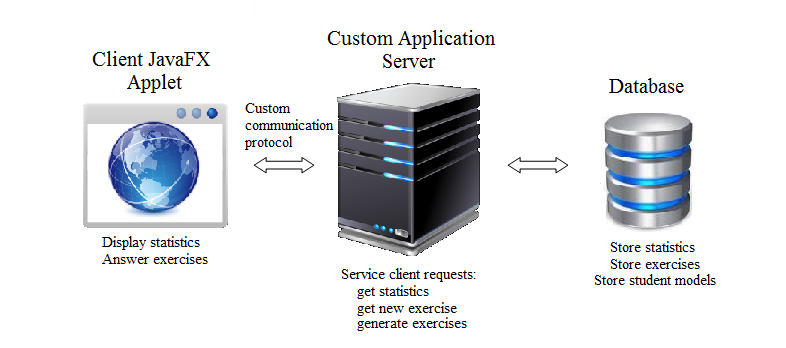
\includegraphics[width=\textwidth,height=\textheight,keepaspectratio]{three-tier-architecture}
\caption{Three tier architecture of the jSCAPE system.}
\label{fig:three-tier-architecture}
\end{figure}


CAT development, we refer back to the five components of a CAT...what item selection algorithm we use, what scoring procedure, no termination criterion, entry point is average knowledge distribution initially and attempts at a calibrated item pool, currently with teacher providing the parameters since obtaining a high quality calibrated item pool isn't something I can do.
\newpage

\lstinputlisting[caption={Item information algorithm.}]{\listings/item_information.java}

\newpage

\lstinputlisting[caption={Item response function algorithm.}]{\listings/item_response_function.java}

\newpage
\lstinputlisting[caption={Example exercise illustrating the XML format.}]{\listings/exercise.xml}

\begin{figure}[H]
\centering
\begin{tikzpicture}[>=stealth',shorten >=1pt,auto,node distance=3cm]
  \node[initial,state] (A1)      {$A1$};
  \node[state]         (A2) [right of=A1]  {$A2$};
  \node[state]         (A3) [right of=A2] {$A3$};
  \node[state]         (B1) [below of=A3] {$B1$};
  \node[state]         (B2) [left of=B1] {$B2$};
  \node[state]         (B3) [left of=B2] {$B3$};
  \node[state]         (C1) [below of=B3] {$C1$};
  \node[state]         (C2) [right of=C1] {$C2$};
  \node[state]         (C3) [right of=C2] {$C3$};


  \path[->] (A1)  edge [loop above] node {wrong} (A1)
             edge [bend left] node {correct} (A2)
        (A2) edge [bend left]  node {wrong} (A1)
             edge [bend left] node {correct} (A3)
        (A3) edge [bend left]  node {wrong} (A2)
             edge [bend left] node {correct} (B1)
        (B1) edge [bend left]  node {wrong} (A3)
             edge [bend left] node {correct} (B2)
        (B2) edge [bend left]  node {wrong} (B1)
             edge [bend left] node {correct} (B3)
        (B3) edge [bend left] node {wrong} (B2)
             edge [bend left] node {correct} (C1)
        (C1) edge [bend left] node {wrong} (B3)
             edge [bend left] node {correct} (C2)
        (C2) edge [bend left] node {wrong} (C1)
             edge [bend left] node {correct} (C3)
        (C3) edge [loop above] node {correct} (C3)
             edge [bend left] node {wrong} (C2);             
\end{tikzpicture}
\caption{State machine of adaptive difficulty categories.}
\label{state-machine}
\end{figure}